\section{Lemmatization and part-of-speech tagging}
\label{chap:tag}
Lemmatization and \acrlong{pos} tagging tasks are often categorized as morphological analysis, shares same architecture and trained network, so they will be described together in this section.
\subsection{Task Definition}
%co chci presne delat - vstup, vystup, metrika

\paragraph{\textbf{POS tagging}} \mbox{}\\
\textit{input}: a word \\
\textit{output}: tag, which contains not only part-of-speech (e.g. noun, pronoun, punctuation mark) but also other morphological analysis (case, tense, etc) corresponding to 15-places morphological tagging system by \cite{Hajic2004}. Description of each position can be found in Table \ref{Tab:tagset}.

\paragraph{\textbf{Lemmatization}} \mbox{}\\
\textit{input:} a word \\
\textit{output:} lemma -- a base form of a given words, meaning for example nominative of singular for nouns or infinitive for verbs. In this work, lemmatization is treated as a classification problem with classes coresponding to generating rules which transform an input word into target lemma. For example of such rules see Figure \ref{fig:lemma_rules}. \\


Metric used for evaluation of the model is an accuracy reported separately for several options -- only tags/lemmas, accuracy of joint classification of tags and lemmas, and  also for all variants with an usage of dictionary (this option is described in more detail in \ref{sub:dataset}).

\begin{figure}[H]
\centering
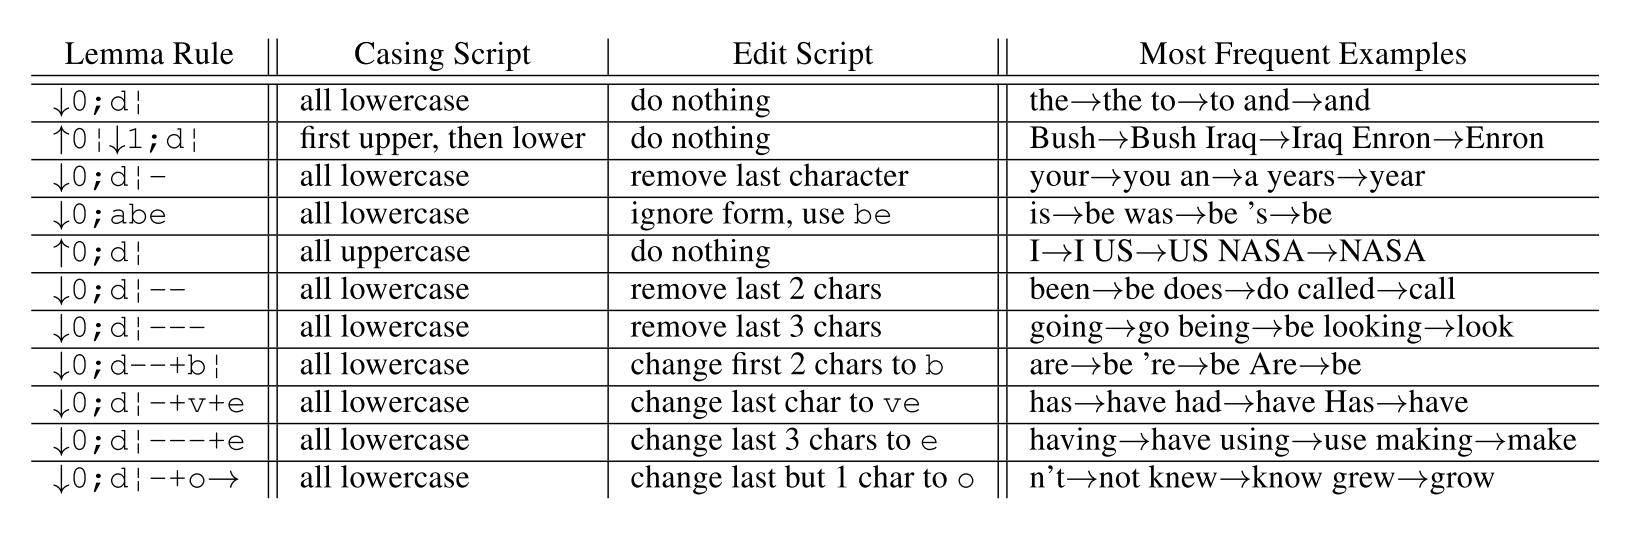
\includegraphics[width=1\textwidth]{../img/lemma_rules}
\protect\caption{
Table 1 from \citep{Straka2019b} presents 10 most common lemma generating rules in English EWT corpus. Each rule has two parts -- casing script for transforming uppercase and lowercase letters, and edit script. Edit script can transform prefix, suffix, or also a root of the word.
}
\label{fig:lemma_rules}
\end{figure}

\begin{table}
\centering
\label{Tab:tagset}
\begin{tabular}{ |c|c|c| } 

 \hline
 Position & Name & Description \\ 
 \hline \hline
 1 & POS & Part of speech \\ \hline
 2 & SubPOS & Detailed part of speech \\ \hline
  3 & Gender & Gender \\ \hline
4 & Number & Number \\\hline
  5 & Case & Case \\ \hline
 6 & PossGender & Possessor's gender \\\hline
  7 & PossNumber & Possessor's number \\ \hline
8 & Person & Person \\\hline
  9 & Tense & Tense \\ \hline
 10 & Grade & Degree of comparison\\\hline
  11 & Negation & Negation \\ \hline
 12 & Voice & Voice \\\hline
 13 & Reserve1 & Reserve \\ \hline
14 & Reserve2 & Reserve \\\hline
  15 & Var & Variant, style \\ 
 \hline

\end{tabular}
\caption{Czech morphology developement is dated from 1989 \citep{Hajic2004} %TODO zdroj Hajič
and in description of words uses 15-places morphological tags as described in this table taken from https://ufal.mff.cuni.cz/pdt2.0/doc/manuals/en/m-layer/html/ch02s02s01.html}
\end{table}

\subsection{Related Work}
This work aims to improve previously published SOTA results for contextualized embeddings in czech lemmatization and tagging \citep{Straka2019}. 

as described in table \ref{Tab:tagset}.  %TODO a ja pouzivam ty samy? 


%\citep{Horsmann}
%\citep{Plank}
%\citep{Plisson}
%\citep{Straka2019b}
%\citep{Straka2019a}
%\citep{Toutanova2003}
%\citep{Wang2015}
%\citep{Huang2015}
%\citep{Collobert2011} ... preprocessing

\subsection{Dataset and Preprocessing}
\label{sub:dataset}
%TODO popisje v straka2019 - dopnit
Dataset for these tasks is taken from data of Prague Dependency Treebank (PDT) \citep{PDT35}, specifically version 3.5, which is PDT version from year 2018. %Dataset is divided into three parts - train, developement and test.  %TODO jak vypadaji vstupni data - ukazka z tech dat co mam primo!!!
Data consists of sentences with lemmas and tags. For ambiguous words, data contain all possible analysis. For example, Czech word "psa" have one possible lemma ("pes") but two possible tags because it could be one of two possible grammatical cases -- genitive or accusative. Input data for such word looks as follows: \\
\begin{center}
psa pes NNMS2-----A---- NNMS4-----A----
\end{center}.

Dataset was originally divided into tree parts - train, development and test, which is also used in this work. Input sentences are preprocessed as follows: %TODO mozna az do site? opsat vse z UDPipe2.0 !!!
\begin{itemize}
\item white space deletion
\item splitting into sentences and words
\item mapping characters and words into numbers -- mapping  words/characters which were found in train dataset into integers (from one to the number of unique words). This means, that the network has no information about words/characters which appears only in test or development dataset. All newly appeared words/characters are mapped into one same number (typically $0$) for \textit{UNK} token/character.
\item tokenization -- Tokenizer for corresponding BERT-like model transforms input words into tokens. Each word is transformed into one or more strings, which are converted into numbers. This serves as an input into BERT part of model. To creating these input embeddings, the whole sentence for each word is needed as same words can have different representation in different contexts. More information can be found in\ref{sub:tokens}.
\end{itemize}

\subsection{Experiments and Architecture}

%For POS tagging, we applied a straightforward model in the lines of Ling et al. (2015) – first rep- resenting each word with its embedding, contextu- alizing them with bidirectional RNNs (Graves and Schmidhuber, 2005), and finally using a softmax classifier to predict the tags. z UDpipe2

%??? We perform tokenization, sentence segmentation and multi-word token splitting with the baseline UDPipe 1.2 approach. In a nutshell, input charac- ters are first embedded using trained embeddings, then fixed size input segments (of 50 characters) are processed by a bidirectional GRU (Cho et al., 2014), and each character is classified into three classes – a) there is a sentence break after this character, b) there is a token break after this char- acter, and c) there is no break after this character.

%reprezentation: tři typy embeddings - pretrained, trained, character-level a ještě berti

%TODO popisovat vice ty pravidla?

The model for lemmatization and tagging is build upon a model (and a code) for previous work on Czech NLP processing with contextual embeddings \citep{straka2019czech}. Data preprocessing is taken over from the paper as well as the structure of a lemmatizer and a tagger network which is extended by BERT-like models,hoping for improvements. Previous work \citep{Straka2019}, \citep{Straka2018} showed that training tagging and lemmatization together in one network can be mutually advantageous, soboth of these analysis are an output of one network and are trained jointly. Detailed visualisation of network architecture can aslo be found in Figure \ref{pic:lt_arch}. \par
The architecture of network can be divided into three parts -- inputs, optional \acrshort{rnn}s, classification head.
\paragraph{Inputs}
An input of the network is formed of five types -- characters (charseqs), words (charseq ids), correct responses(word ids), pretrained embeddings and possibly precomputed bert embeddings (depends on the experiment type). Before the further processing of inputs by \acrshort{rnn} cells, there are created two other types of embeddings: character-level embeddings and another word embeddings which are, in contrast to BERT and pretrained embeddings, also trained during training process.

\paragraph{RNN cells}
Characterlevel embeddings are further processed via \acrfull{gru} and all inputs (or their embeddings) are processed by recurrent part of network (specifically by \acrfull{lstm} cells).

\paragraph{Outputs}
After the processing by recurrent neural networks, network employs two separate classification head, one for tagging and another for lemmatization. Both uses dense layer with tanh activation function to presented more non-linearity as used in \citep{2018} and a softmax function for obtaining the probability distribution over target classes. Lemmatization, however, presents one another change -- addition of character level data without RNN processing, which are used together with the rest of weights as an input into softmax following \citep{Straka2018}, because it leads to better performance of lemmatization in the case of shared network between both tasks.

\begin{figure}[ht]
\centering
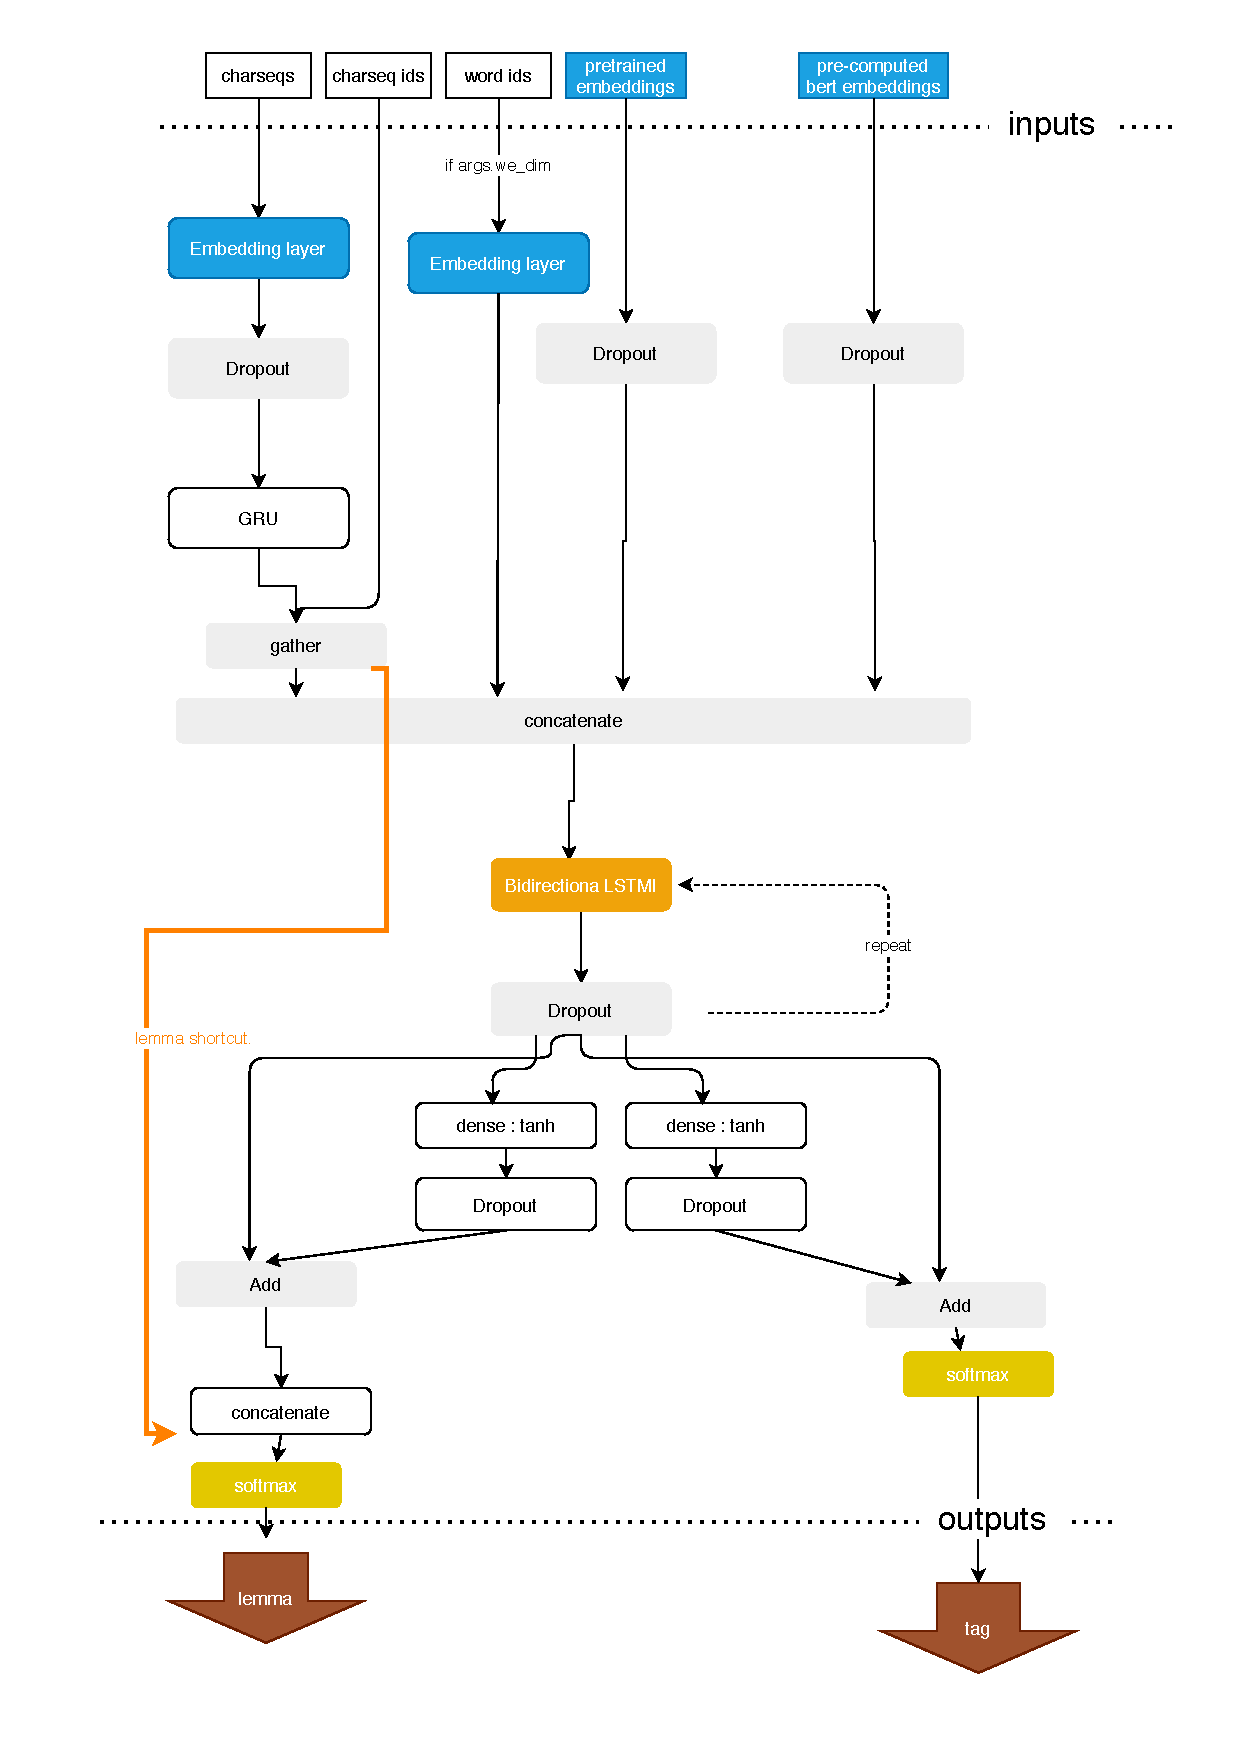
\includegraphics[width=1\columnwidth]{../img/taggermodel.pdf}
\protect\caption{popis? }
\label{pic:lt_arch}
\end{figure}

\paragraph{Morphological Dictionary} All classification can be done with or without use of a morphological dictionary MorFlex \citep{11234/1-1834}, which can provide possible pairs (tag, lemma). If so, generated tags and lemmas are chosen just from the dictionary. So it is selected lemma and/or tag with maximal likelihood, but only one from those presented in the dictionary. 

\subsubsection{Experiments}
%TODO jake modely
\begin{itemize}
\item baseline solution -- reimplementation of \citep{Straka2019czech} without/with label smoothing,
\item precomputed BERT embeddings are provided as as another static input of the model, 
\item finetunning of precomputed BERT embeddings -- after perfoming
\end{itemize}





\subsection{Results}

\begin{table}[!h]
  \begin{tabular}{|l||c|c|c||c|c|c|}
  \hline
\multirow{2}{*}{Experiment} & \multicolumn{3}{c||}{Without Dictionary}  &
      \multicolumn{3}{c|}{With Dictionary} \\ 
    & Tags & Lemmas & Both & Tags & Lemmas & Both \\ \hline
    StrakaB & 97.94\% & 98.75\% & 97.31\% & 98.05\% & 98.98\% & 97.65\% \\ \hline
    emb (lr 0.0001) &  97.80\% & 98.70\% & 97.17\% & 97.95\% & 98.93\% & 97.55\% \\ \hline
    baseline & 97.04 \% & 98.56 \% & 96.41\% &  97.31  \% & 98.83 \% & 96.90\% \\ \hline 
    StrakaC & 97.67\% & 98.63\% & 97.02\% & 97.91\% & 98.94\% & 97.51\% \\ \hline
  \end{tabular}
  \caption{%TODO cite
  Straka2019B is the best solution from \citep{Straka2019} paper. Straka2019C is a comparable solution  (BERT embeddings only), which was transformed into TF2 in this work.} 
\end{table}


